% Options for packages loaded elsewhere
\PassOptionsToPackage{unicode}{hyperref}
\PassOptionsToPackage{hyphens}{url}
%
\documentclass[
  ignorenonframetext,
]{beamer}
\usepackage{pgfpages}
\setbeamertemplate{caption}[numbered]
\setbeamertemplate{caption label separator}{: }
\setbeamercolor{caption name}{fg=normal text.fg}
\beamertemplatenavigationsymbolsempty
% Prevent slide breaks in the middle of a paragraph
\widowpenalties 1 10000
\raggedbottom
\setbeamertemplate{part page}{
  \centering
  \begin{beamercolorbox}[sep=16pt,center]{part title}
    \usebeamerfont{part title}\insertpart\par
  \end{beamercolorbox}
}
\setbeamertemplate{section page}{
  \centering
  \begin{beamercolorbox}[sep=12pt,center]{part title}
    \usebeamerfont{section title}\insertsection\par
  \end{beamercolorbox}
}
\setbeamertemplate{subsection page}{
  \centering
  \begin{beamercolorbox}[sep=8pt,center]{part title}
    \usebeamerfont{subsection title}\insertsubsection\par
  \end{beamercolorbox}
}
\AtBeginPart{
  \frame{\partpage}
}
\AtBeginSection{
  \ifbibliography
  \else
    \frame{\sectionpage}
  \fi
}
\AtBeginSubsection{
  \frame{\subsectionpage}
}
\usepackage{amsmath,amssymb}
\usepackage{lmodern}
\usepackage{ifxetex,ifluatex}
\ifnum 0\ifxetex 1\fi\ifluatex 1\fi=0 % if pdftex
  \usepackage[T1]{fontenc}
  \usepackage[utf8]{inputenc}
  \usepackage{textcomp} % provide euro and other symbols
\else % if luatex or xetex
  \usepackage{unicode-math}
  \defaultfontfeatures{Scale=MatchLowercase}
  \defaultfontfeatures[\rmfamily]{Ligatures=TeX,Scale=1}
  \setmainfont[BoldFont = SF Pro Rounded Semibold]{SF Pro Rounded}
  \setmathfont[]{STIX Two Math}
\fi
\usefonttheme{serif} % use mainfont rather than sansfont for slide text
% Use upquote if available, for straight quotes in verbatim environments
\IfFileExists{upquote.sty}{\usepackage{upquote}}{}
\IfFileExists{microtype.sty}{% use microtype if available
  \usepackage[]{microtype}
  \UseMicrotypeSet[protrusion]{basicmath} % disable protrusion for tt fonts
}{}
\makeatletter
\@ifundefined{KOMAClassName}{% if non-KOMA class
  \IfFileExists{parskip.sty}{%
    \usepackage{parskip}
  }{% else
    \setlength{\parindent}{0pt}
    \setlength{\parskip}{6pt plus 2pt minus 1pt}}
}{% if KOMA class
  \KOMAoptions{parskip=half}}
\makeatother
\usepackage{xcolor}
\IfFileExists{xurl.sty}{\usepackage{xurl}}{} % add URL line breaks if available
\IfFileExists{bookmark.sty}{\usepackage{bookmark}}{\usepackage{hyperref}}
\hypersetup{
  pdftitle={305 Lecture 5.6 - Two Special Cases},
  pdfauthor={Brian Weatherson},
  hidelinks,
  pdfcreator={LaTeX via pandoc}}
\urlstyle{same} % disable monospaced font for URLs
\newif\ifbibliography
\usepackage{graphicx}
\makeatletter
\def\maxwidth{\ifdim\Gin@nat@width>\linewidth\linewidth\else\Gin@nat@width\fi}
\def\maxheight{\ifdim\Gin@nat@height>\textheight\textheight\else\Gin@nat@height\fi}
\makeatother
% Scale images if necessary, so that they will not overflow the page
% margins by default, and it is still possible to overwrite the defaults
% using explicit options in \includegraphics[width, height, ...]{}
\setkeys{Gin}{width=\maxwidth,height=\maxheight,keepaspectratio}
% Set default figure placement to htbp
\makeatletter
\def\fps@figure{htbp}
\makeatother
\setlength{\emergencystretch}{3em} % prevent overfull lines
\providecommand{\tightlist}{%
  \setlength{\itemsep}{0pt}\setlength{\parskip}{0pt}}
\setcounter{secnumdepth}{-\maxdimen} % remove section numbering
\let\Tiny=\tiny

 \setbeamertemplate{navigation symbols}{} 

% \usetheme{Madrid}
 \usetheme[numbering=none, progressbar=foot]{metropolis}
 \usecolortheme{wolverine}
 \usepackage{color}
 \usepackage{MnSymbol}
% \usepackage{movie15}

\usepackage{amssymb}% http://ctan.org/pkg/amssymb
\usepackage{pifont}% http://ctan.org/pkg/pifont
\newcommand{\cmark}{\ding{51}}%
\newcommand{\xmark}{\ding{55}}%

\DeclareSymbolFont{symbolsC}{U}{txsyc}{m}{n}
\DeclareMathSymbol{\boxright}{\mathrel}{symbolsC}{128}
\DeclareMathAlphabet{\mathpzc}{OT1}{pzc}{m}{it}

\usepackage{tikz-qtree}
% \usepackage{markdown}
%\RequirePackage{bussproofs}
\usetikzlibrary{arrows.meta}
\RequirePackage[tableaux]{prooftrees}
\forestset{line numbering, close with = x}
% Allow for easy commas inside trees
\renewcommand{\,}{\text{, }}


\usepackage{tabulary}

\usepackage{open-logic-config}

\setlength{\parskip}{1ex plus 0.5ex minus 0.2ex}

\AtBeginSection[]
{
\begin{frame}
	\Huge{\color{darkblue} \insertsection}
\end{frame}
}

\renewenvironment*{quote}	
	{\list{}{\rightmargin   \leftmargin} \item } 	
	{\endlist }

\definecolor{darkgreen}{rgb}{0,0.7,0}
\definecolor{darkblue}{rgb}{0,0,0.8}

\newcommand{\starttab}{\begin{center}
\vspace{6pt}
\begin{tabular}}

\newcommand{\stoptab}{\end{tabular}
\vspace{6pt}
\end{center}
\noindent}


\newcommand{\sif}{\rightarrow}
\newcommand{\siff}{\leftrightarrow}
\newcommand{\EF}{\end{frame}}


\newcommand{\TreeStart}[1]{
%\end{frame}
\begin{frame}
\begin{center}
\begin{tikzpicture}[scale=#1]
\tikzset{every tree node/.style={align=center,anchor=north}}
%\Tree
}

\newcommand{\TreeEnd}{
\end{tikzpicture}
%\end{center}
}

\newcommand{\DisplayArg}[2]{
\begin{enumerate}
{#1}
\end{enumerate}
\vspace{-6pt}
\hrulefill

%\hspace{14pt} #2
%{\addtolength{\leftskip}{14pt} #2}
\begin{quote}
{\normalfont #2}
\end{quote}
\vspace{12pt}
}

\newenvironment{ProofTree}[1][1]{
\begin{center}
\begin{tikzpicture}[scale=#1]
\tikzset{every tree node/.style={align=center,anchor=south}}
}
{
\end{tikzpicture}
\end{center}
}

\newcommand{\TreeFrame}[2]{
\begin{columns}[c]
\column{0.5\textwidth}
\begin{center}
\begin{prooftree}{}
#1
\end{prooftree}
\end{center}
\column{0.45\textwidth}
%\begin{markdown}
#2
%\end{markdown}
\end{columns}
}

\newcommand{\ScaledTreeFrame}[3]{
\begin{columns}[c]
\column{0.5\textwidth}
\begin{center}
\scalebox{#1}{
\begin{prooftree}{}
#2
\end{prooftree}
}
\end{center}
\column{0.45\textwidth}
%\begin{markdown}
#3
%\end{markdown}
\end{columns}
}

\usepackage[bb=boondox]{mathalfa}
\DeclareMathAlphabet{\mathbx}{U}{BOONDOX-ds}{m}{n}
\SetMathAlphabet{\mathbx}{bold}{U}{BOONDOX-ds}{b}{n}
\DeclareMathAlphabet{\mathbbx} {U}{BOONDOX-ds}{b}{n}


\newenvironment{oltableau}{\center\tableau{}} %wff format={anchor = base west}}}
       {\endtableau\endcenter}
       
\newcommand{\formula}[1]{$#1$}

\usepackage{tabulary}
\usepackage{booktabs}

\def\begincols{\begin{columns}}
\def\begincol{\begin{column}}
\def\endcol{\end{column}}
\def\endcols{\end{columns}}

\usepackage[italic]{mathastext}
\usepackage{nicefrac}

\definecolor{mygreen}{RGB}{0, 100, 0}
\definecolor{mypink2}{RGB}{219, 48, 122}
\definecolor{dodgerblue}{RGB}{30,144,255}

%\def\True{\textcolor{dodgerblue}{\text{T}}}
%\def\False{\textcolor{red}{\text{F}}}

\def\True{\mathbb{T}}
\def\False{\mathbb{F}}

% This is because arguments didn't have enough space after them
\usepackage{etoolbox}
\AfterEndEnvironment{description}{\vspace{9pt}}
\AfterEndEnvironment{oltableau}{\vspace{9pt}}
\BeforeBeginEnvironment{oltableau}{\vspace{9pt}}
\AfterEndEnvironment{center}{\vspace{12pt}}
\BeforeBeginEnvironment{tabular}{\vspace{9pt}}

\setlength\heavyrulewidth{0pt}
\setlength\lightrulewidth{0pt}

%\def\toprule{}
%\def\bottomrule{}
%\def\midrule{}

\setbeamertemplate{caption}{\raggedright\insertcaption}

\ifluatex
  \usepackage{selnolig}  % disable illegal ligatures
\fi

\title{305 Lecture 5.6 - Two Special Cases}
\author{Brian Weatherson}
\date{}

\begin{document}
\frame{\titlepage}

\begin{frame}{Plan}
\protect\hypertarget{plan}{}
This lecture looks at two tricky cases, and how the proofs for them
work.
\end{frame}

\begin{frame}{Associated Reading}
\protect\hypertarget{associated-reading}{}
forall x, chapter 17.
\end{frame}

\begin{frame}{Disjunctive Syllogism}
\protect\hypertarget{disjunctive-syllogism}{}
\begin{enumerate}
\tightlist
\item
  \(A \vee B\)
\item
  \(\neg A\)
\item
  So, \(B\)
\end{enumerate}

That looks pretty good; let's try proving it.
\end{frame}

\begin{frame}{\(A \vee B, \neg A \vdash B\)}
\protect\hypertarget{a-vee-b-neg-a-vdash-b}{}
\begin{figure}
\centering
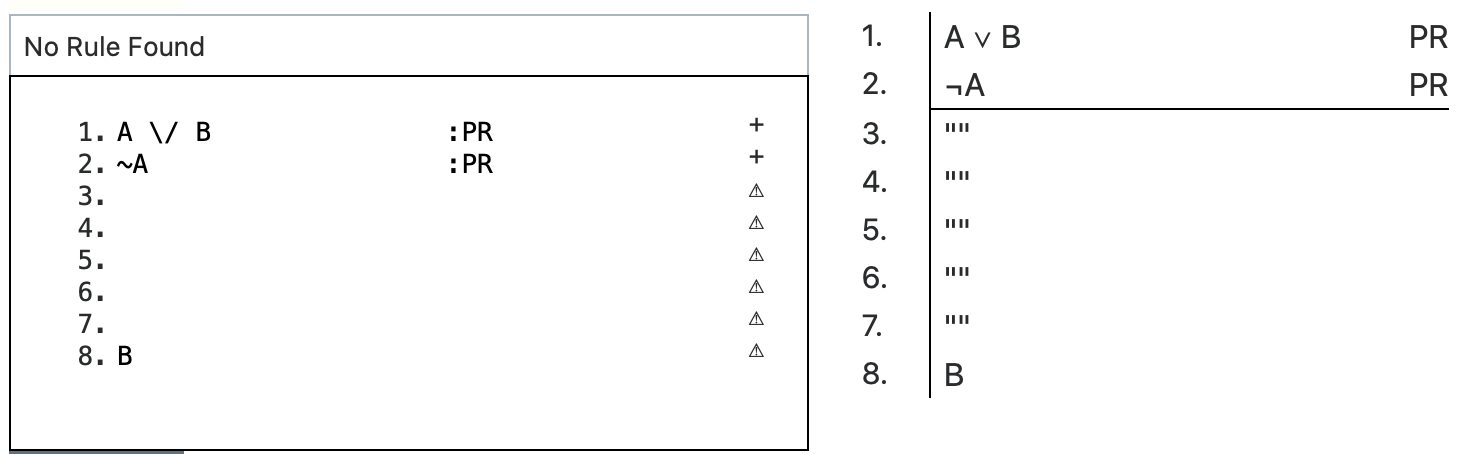
\includegraphics[width=\textwidth,height=0.75\textheight]{5_6a.png}
\caption{List premises and conclusion}
\end{figure}
\end{frame}

\begin{frame}{\(A \vee B, \neg A \vdash B\)}
\protect\hypertarget{a-vee-b-neg-a-vdash-b-1}{}
\begin{figure}
\centering
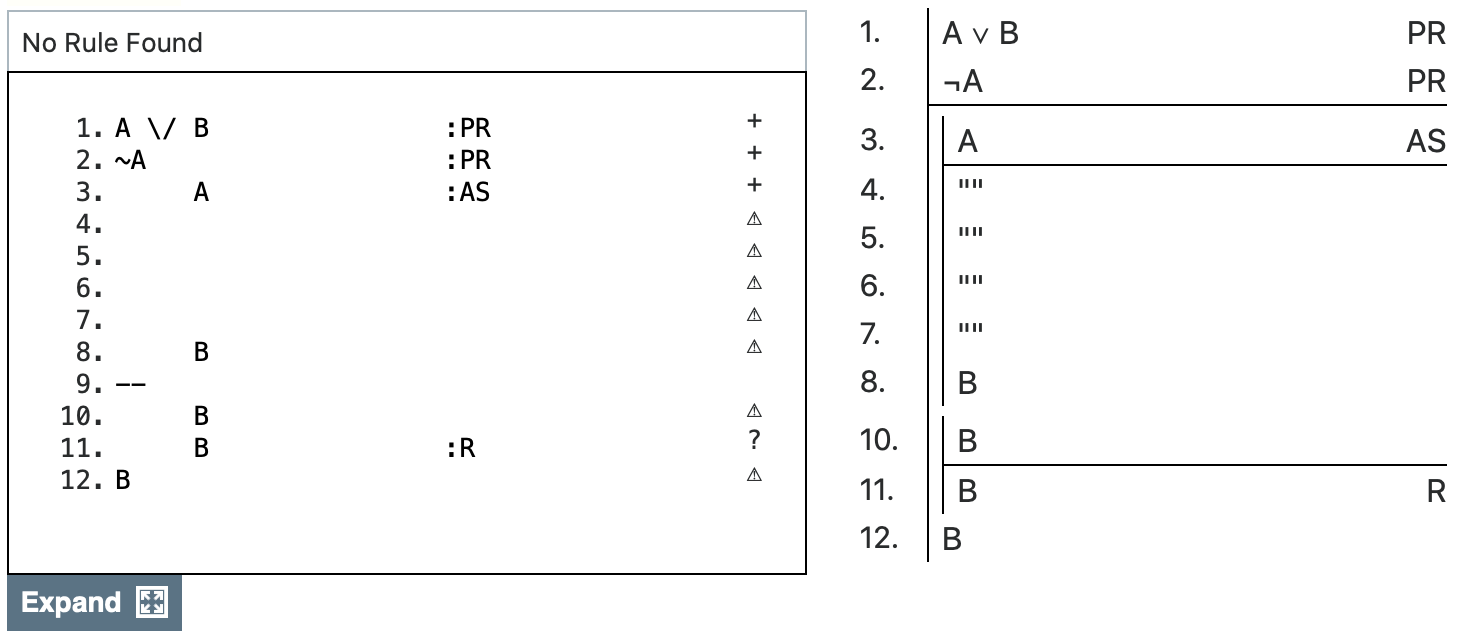
\includegraphics[width=\textwidth,height=0.75\textheight]{5_6b.png}
\caption{We have a \(\vee\) premise, so set up \(\vee\)E}
\end{figure}
\end{frame}

\begin{frame}{\(A \vee B, \neg A \vdash B\)}
\protect\hypertarget{a-vee-b-neg-a-vdash-b-2}{}
\begin{figure}
\centering
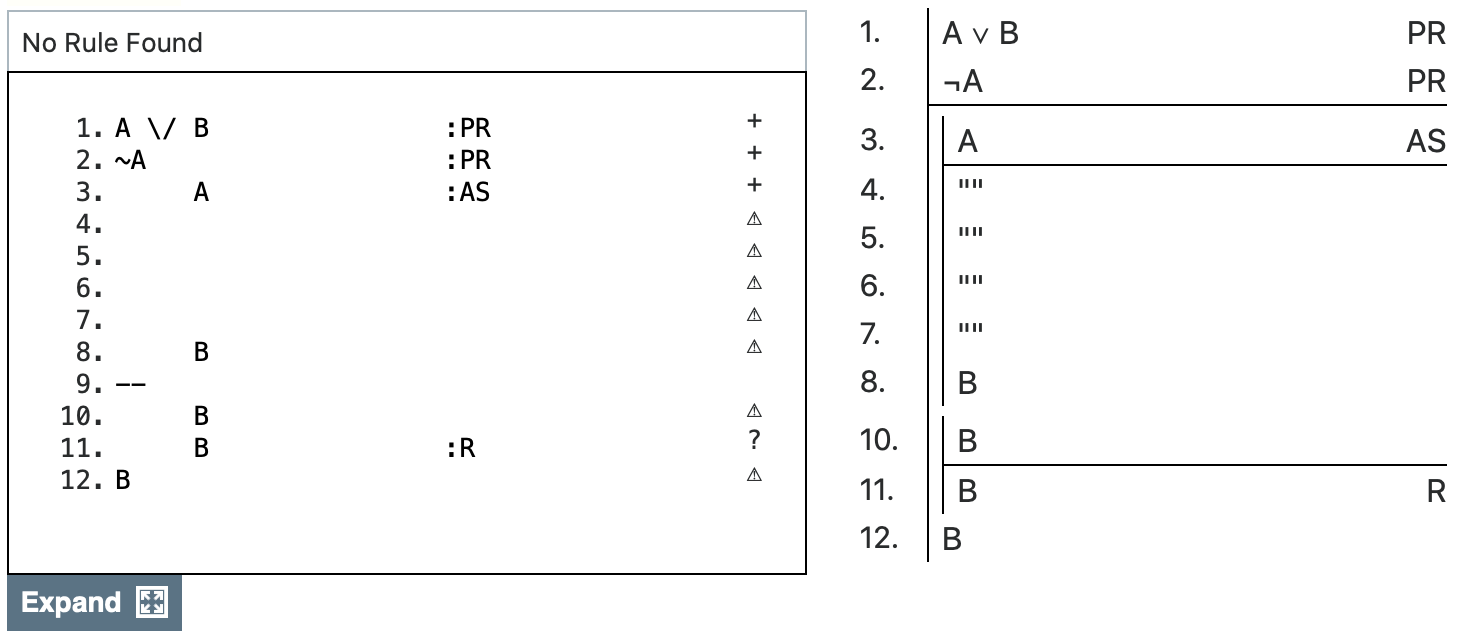
\includegraphics[width=\textwidth,height=0.75\textheight]{5_6b.png}
\caption{I've already added the rule for the second half}
\end{figure}
\end{frame}

\begin{frame}{\(A \vee B, \neg A \vdash B\)}
\protect\hypertarget{a-vee-b-neg-a-vdash-b-3}{}
\begin{figure}
\centering
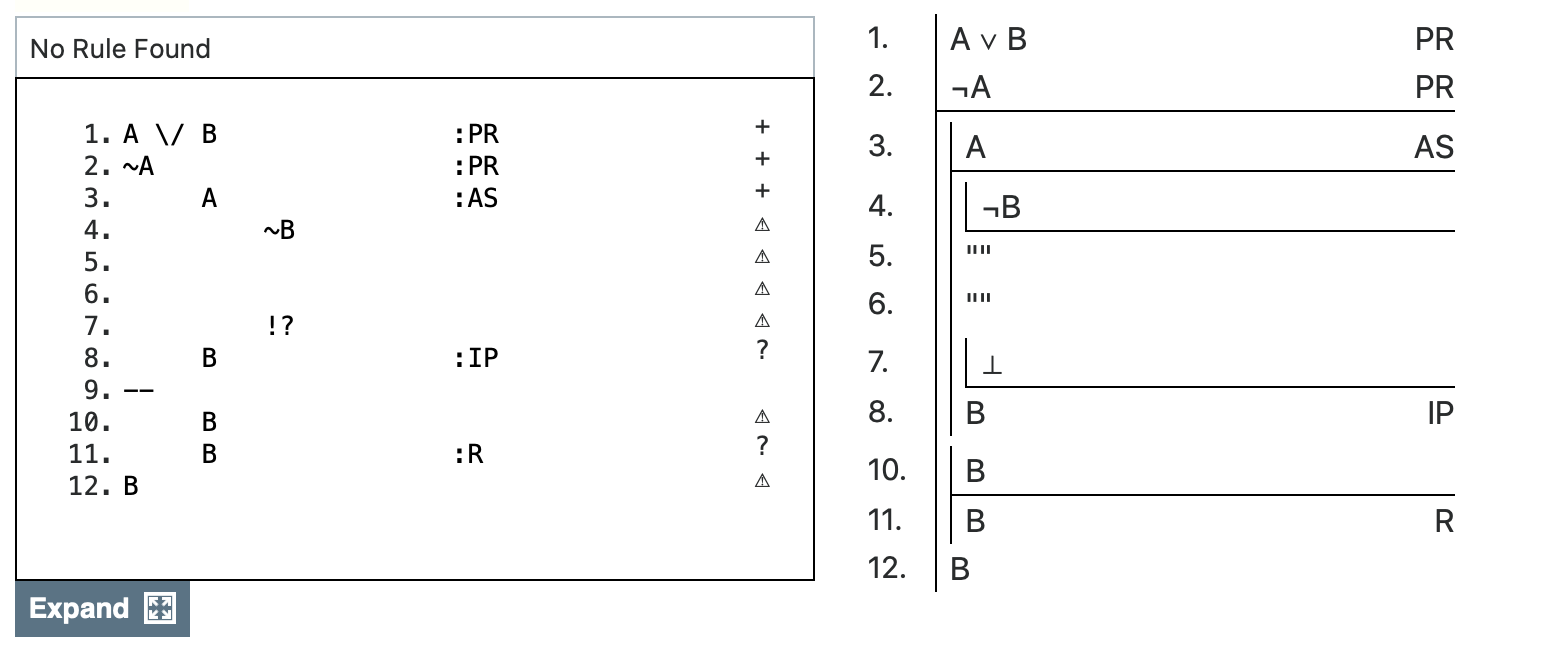
\includegraphics[width=\textwidth,height=0.75\textheight]{5_6c.png}
\caption{A tricky move - we have a \(\neg\) premise so we'll need
Indirect Proof}
\end{figure}
\end{frame}

\begin{frame}{\(A \vee B, \neg A \vdash B\)}
\protect\hypertarget{a-vee-b-neg-a-vdash-b-4}{}
\begin{figure}
\centering
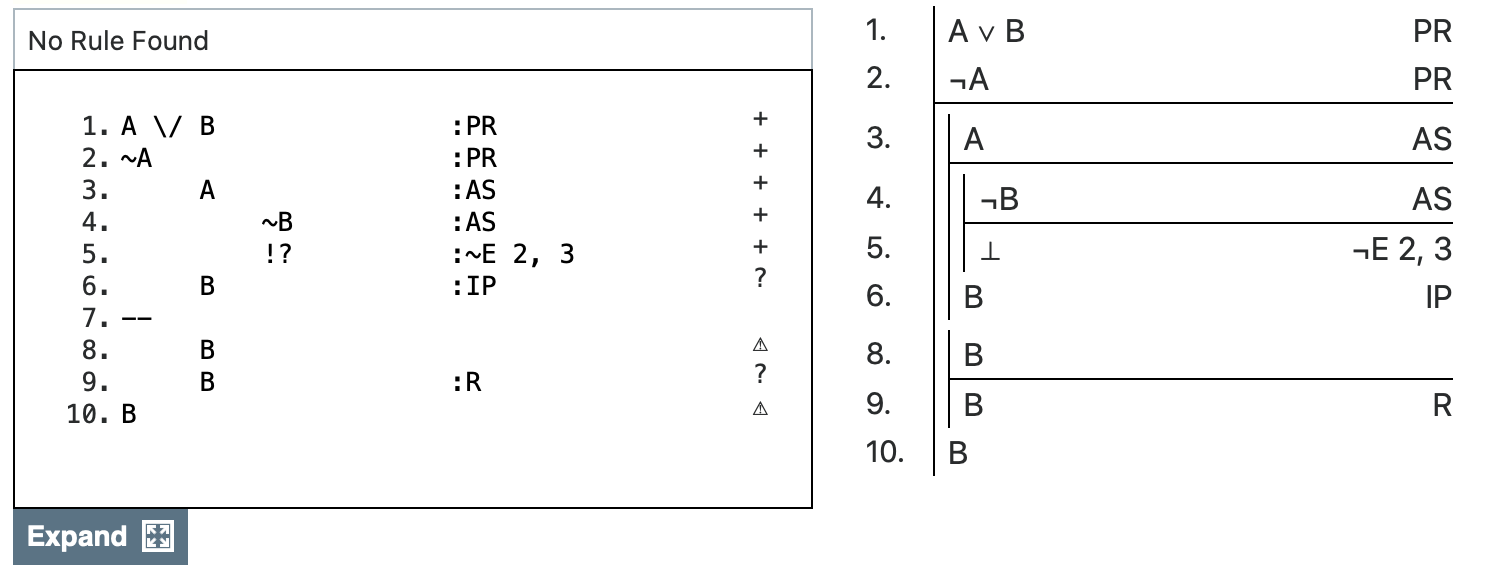
\includegraphics[width=\textwidth,height=0.75\textheight]{5_6d.png}
\caption{And the contradiction comes very easily}
\end{figure}
\end{frame}

\begin{frame}{\(A \vee B, \neg A \vdash B\)}
\protect\hypertarget{a-vee-b-neg-a-vdash-b-5}{}
\begin{figure}
\centering
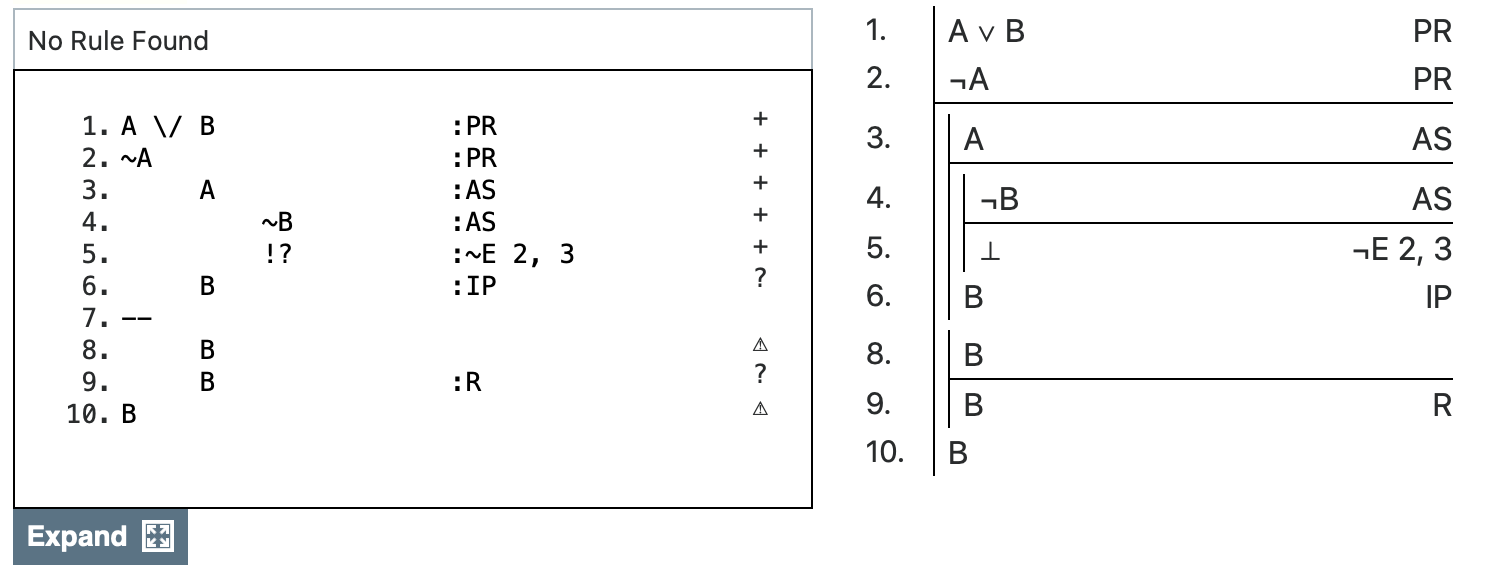
\includegraphics[width=\textwidth,height=0.75\textheight]{5_6d.png}
\caption{Maybe too easily? Should we have been forced to use B?}
\end{figure}
\end{frame}

\begin{frame}{\(A \vee B, \neg A \vdash B\)}
\protect\hypertarget{a-vee-b-neg-a-vdash-b-6}{}
\begin{figure}
\centering
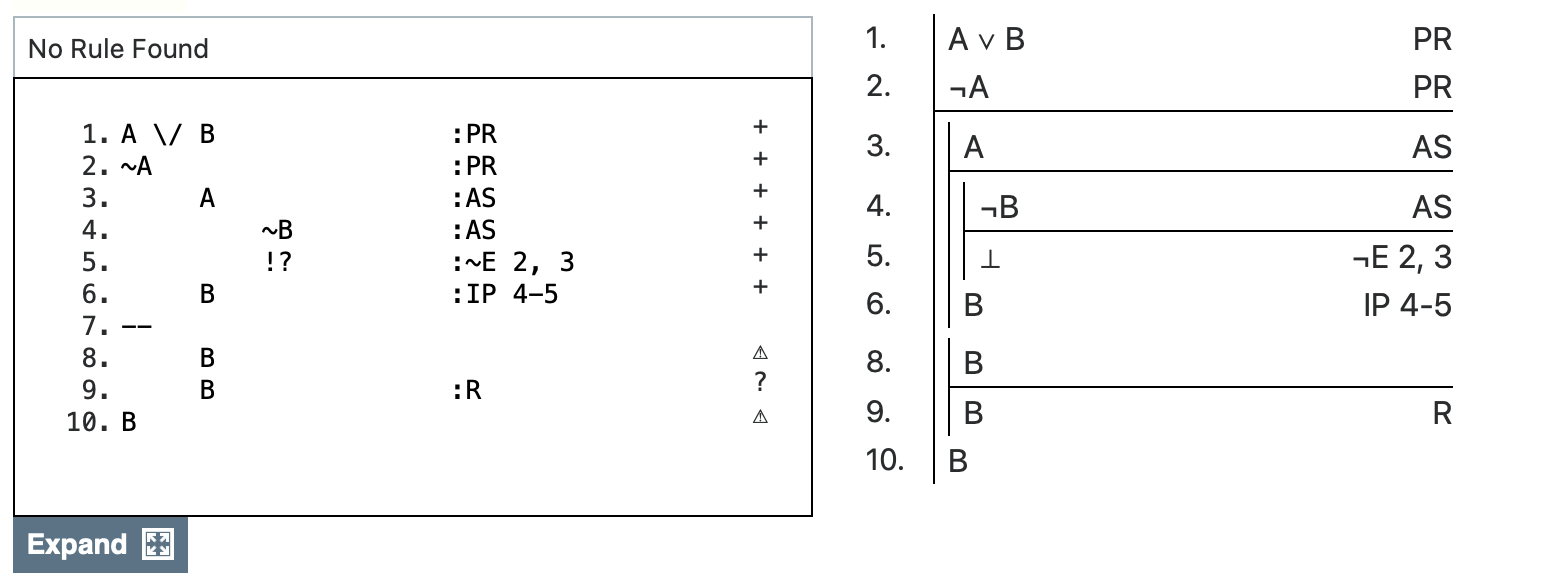
\includegraphics[width=\textwidth,height=0.75\textheight]{5_6e.png}
\caption{Since \(\neg\)B got to contradiction, we can infer B}
\end{figure}
\end{frame}

\begin{frame}{\(A \vee B, \neg A \vdash B\)}
\protect\hypertarget{a-vee-b-neg-a-vdash-b-7}{}
\begin{figure}
\centering
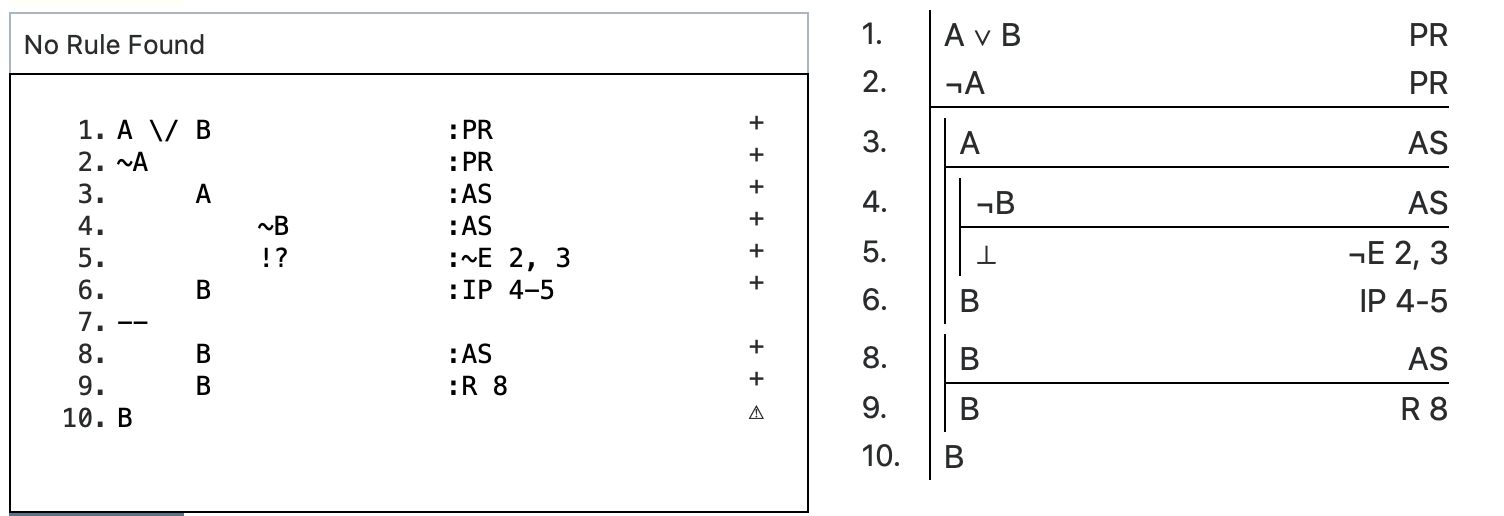
\includegraphics[width=\textwidth,height=0.75\textheight]{5_6g.png}
\caption{Now fill in line number on second subproof}
\end{figure}
\end{frame}

\begin{frame}{\(A \vee B, \neg A \vdash B\)}
\protect\hypertarget{a-vee-b-neg-a-vdash-b-8}{}
\begin{figure}
\centering
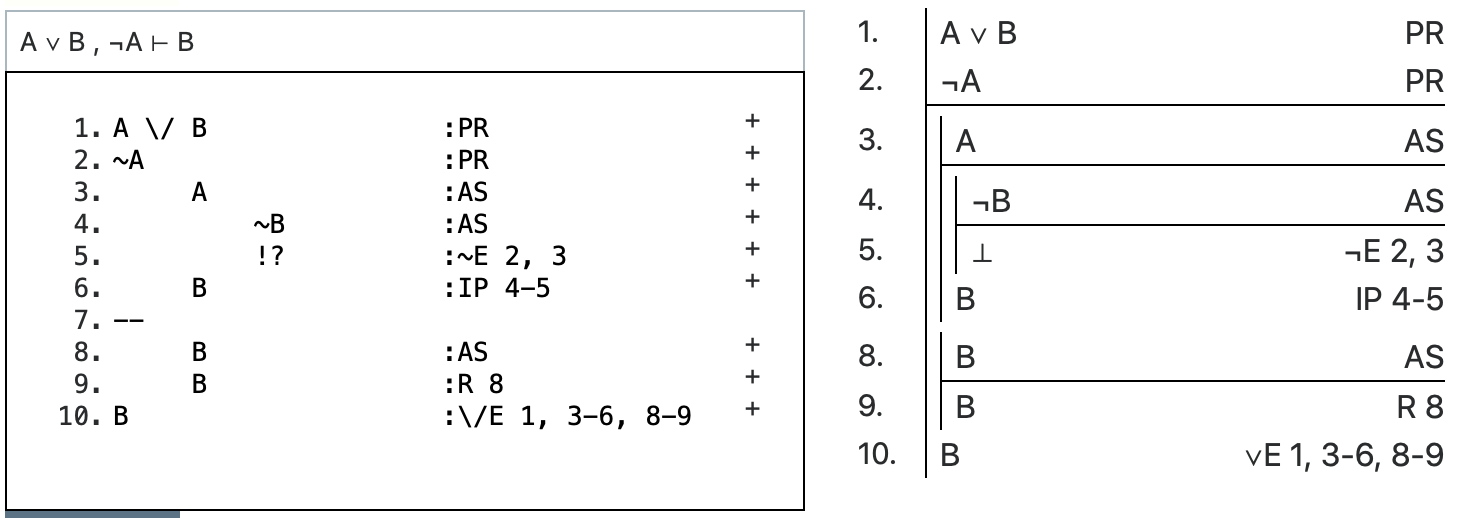
\includegraphics[width=\textwidth,height=0.75\textheight]{5_6h.png}
\caption{And now we're done.}
\end{figure}
\end{frame}

\begin{frame}{Second example}
\protect\hypertarget{second-example}{}
\(\vdash A \vee \neg A\)
\end{frame}

\begin{frame}{How to prove things from zero premises}
\protect\hypertarget{how-to-prove-things-from-zero-premises}{}
\begin{enumerate}
\tightlist
\item
  If they are a conditional, set up \(\rightarrow\)I. The left hand side
  will work just like a premise.
\item
  If they are not a conditional, go for Indirect Proof.
\end{enumerate}
\end{frame}

\begin{frame}{\(\vdash A \vee \neg A\)}
\protect\hypertarget{vdash-a-vee-neg-a}{}
\begin{figure}
\centering
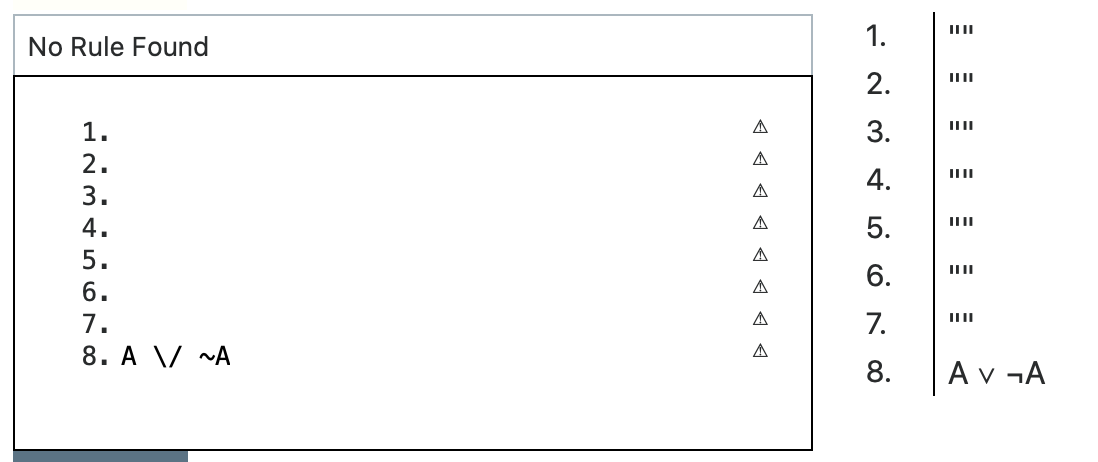
\includegraphics[width=\textwidth,height=0.75\textheight]{5_6p.png}
\caption{Writing out conclusion - but not premise because there is none}
\end{figure}
\end{frame}

\begin{frame}{\(\vdash A \vee \neg A\)}
\protect\hypertarget{vdash-a-vee-neg-a-1}{}
\begin{figure}
\centering
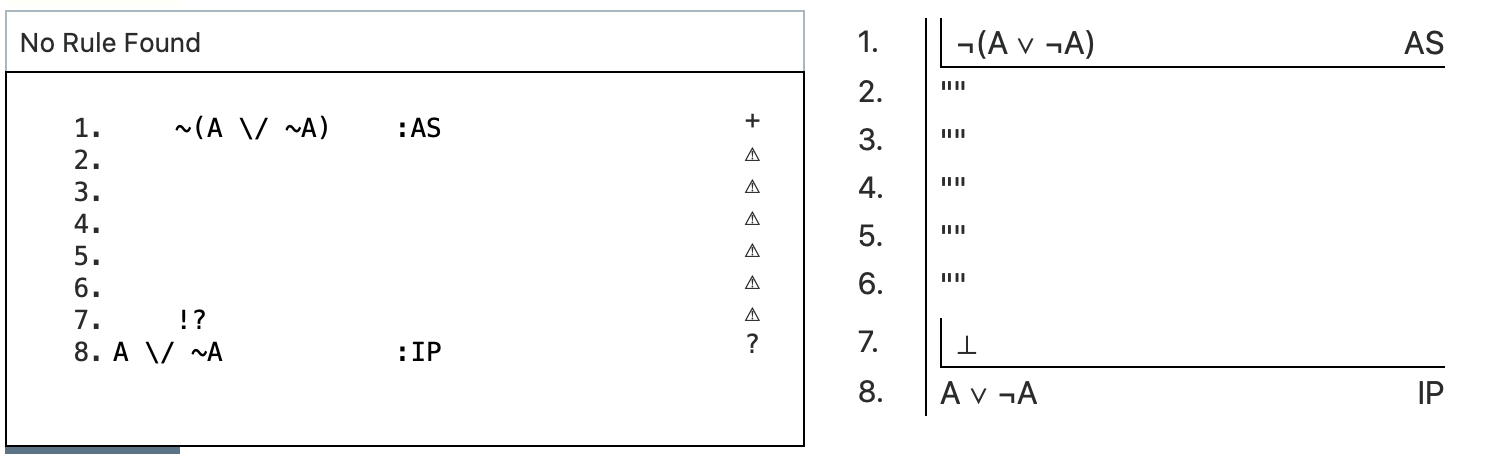
\includegraphics[width=\textwidth,height=0.75\textheight]{5_6q.png}
\caption{Setting up indirect proof}
\end{figure}
\end{frame}

\begin{frame}{\(\vdash A \vee \neg A\)}
\protect\hypertarget{vdash-a-vee-neg-a-2}{}
\begin{figure}
\centering
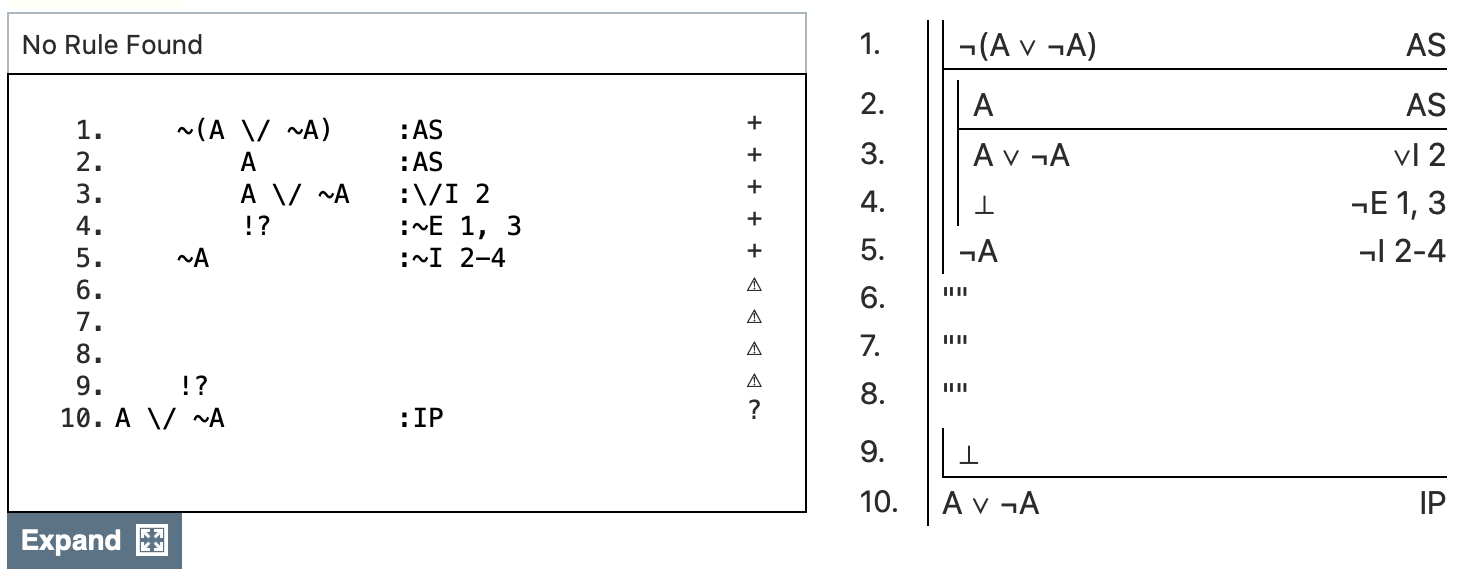
\includegraphics[width=\textwidth,height=0.75\textheight]{5_6r.png}
\caption{A very tricky move - extracting something from negated
disjunction}
\end{figure}
\end{frame}

\begin{frame}{Negated Disjunctions}
\protect\hypertarget{negated-disjunctions}{}
\begin{itemize}
\tightlist
\item
  The move from the previous slide is more or less compulsory.
\item
  The only way to get something out of \(\neg(X \vee Y)\) is to assume
  \(X\), get a contradiction (via deriving \(X \vee Y\)), and then use
  \(\neg\)I to get \(\neg X\).
\item
  It's a pain, and it's just a move you have to learn.
\item
  It might be my single least favorite part of this system.
\end{itemize}
\end{frame}

\begin{frame}{\(\vdash A \vee \neg A\)}
\protect\hypertarget{vdash-a-vee-neg-a-3}{}
\begin{figure}
\centering
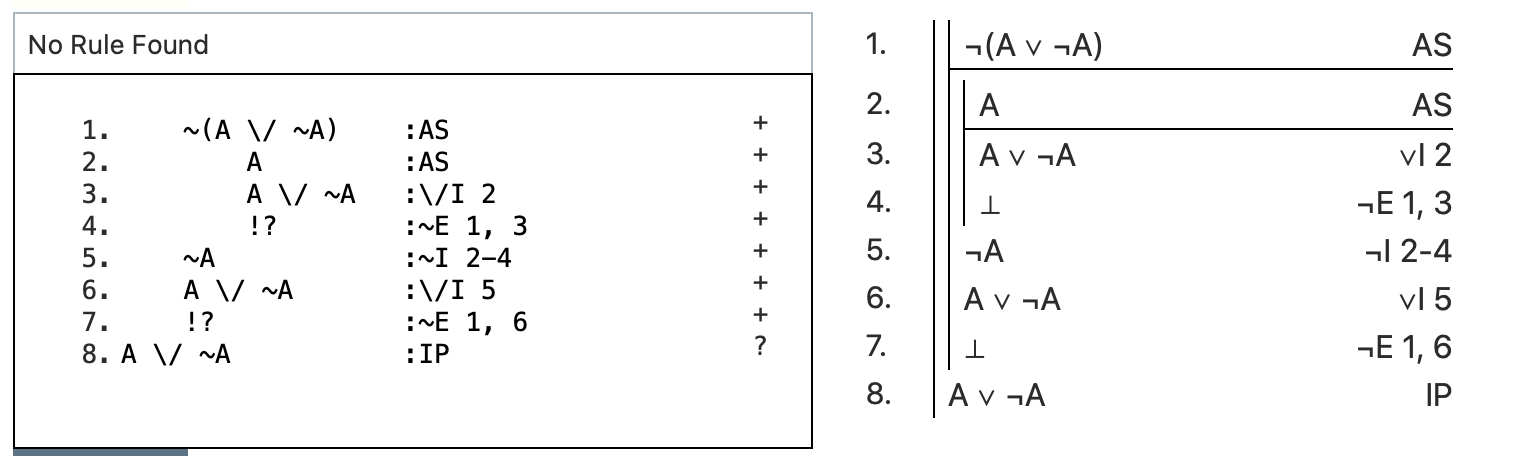
\includegraphics[width=\textwidth,height=0.75\textheight]{5_6s.png}
\caption{If we have \(\neg A\), we are basically home}
\end{figure}
\end{frame}

\begin{frame}{\(\vdash A \vee \neg A\)}
\protect\hypertarget{vdash-a-vee-neg-a-4}{}
\begin{figure}
\centering
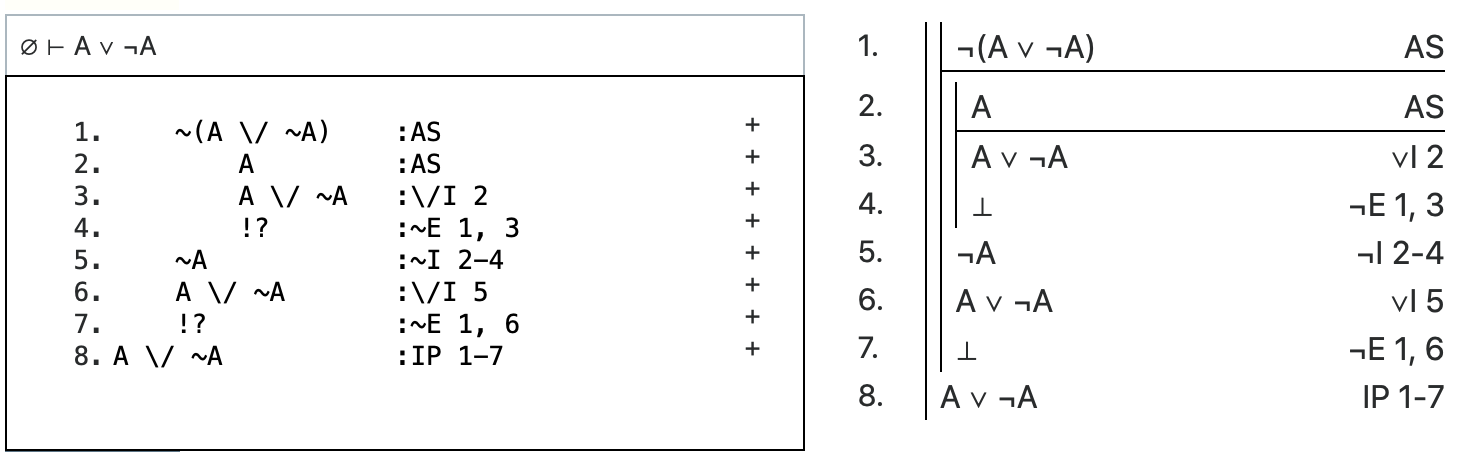
\includegraphics[width=\textwidth,height=0.75\textheight]{5_6t.png}
\caption{Filling in line numbers - note the subproof is the entire proof
to this point}
\end{figure}
\end{frame}

\begin{frame}{Challenge Problem}
\protect\hypertarget{challenge-problem}{}
\begin{enumerate}
\tightlist
\item
  Prove \(\vdash ((A \rightarrow B) \rightarrow A) \rightarrow A\)
\item
  See if you can complete that proof in under 25 lines.
\end{enumerate}

That one, like \(\vdash A \vee \neg A\), is a sign that the strategies
in 17.1 and 17.2 work 98\% of the time, but not 100\% of the time.
\end{frame}

\begin{frame}{For Next Time}
\protect\hypertarget{for-next-time}{}
No recorded lectures next week. We'll just go over the proofs in the
weekly assignment, and do some revision.
\end{frame}

\end{document}
